\chapter{Results}
\label{chap:results}

    By the nature of the defined configurations $\mathcal{C}_i$, the neural network
    \emph{points2mesh} has several reconstructions for each input point cloud $\mathcal{PC}$.
    Since it is not easy to estimate the quality of reconstructed meshes only based on numerical
    values, it is vital to assess their visual quality, tough highly subjective.
    Therefore, in this chapter, a wide range of reconstructed objects of various categories $\mathcal{C}_i$
    are presented and displayed next to their input point cloud $\mathcal{PC}$ and their ground 
    truth mesh. Some interesting features of reconstructions are pointed out, and presented with reconstructions of comparable
    reconstruction methods, as well as the alternative approach to train the network as outline in \ref{trainings}.
    
\section{Compared methods}

Restoring polygonal meshes directly from point cloud data is a new domain of geometry reconstruction, 
which yet has to be explored deeply. Apart from \emph{points2mesh}, no other methods relying on neural 
networks and deep learning techniques have yet been proposed for this kind of mode of data transformation.
For this reason, \emph{points2mesh} has to compete against techniques from traditional approaches like
\emph{ball-pivoting algorithm} \cite{817351}(~BPA~) and \emph{instant field meshes} \cite{Jakob2015Instant} (~IFM~). Furthermore, by adding
an intermediate step of voxelization of $\mathcal{PC}$, this work also can be compared against 
\emph{deep marching cubes} \cite{Liao2018CVPR} (~DMC~), which transforms voxelized data into meshes based on deep learning approaches and the classical
marching cubes algorithm.

\section{Result visualization}
% 1024Figure
  \ref{fig:1} shows the reconstruction from a point cloud sample size of 1024 from the \emph{category}
  \emph{airplane}. \ref{fig:1a} shows the ground truth mesh, and \ref{fig:1d} its sampled point cloud. Figures
  \ref{fig:1b}, \ref{fig:1c}, \ref{fig:1e}, \ref{fig:1f} show the reconstruction from $\mathcal{N}_{recon}$ with 
  configurations $\mathcal{C}_1$ through $\mathcal{C}_4$.

\begin{figure}[htbp]
  \centering
  \subfloat[Ground truth mesh.\label{fig:1a}]{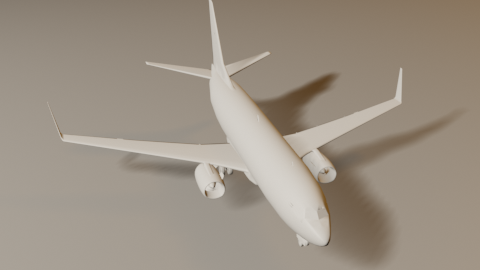
\includegraphics[width=0.32\textwidth]{gt_airplane_1.png}}
  \subfloat[Configuration $\mathcal{C}_1$.\label{fig:1b}]{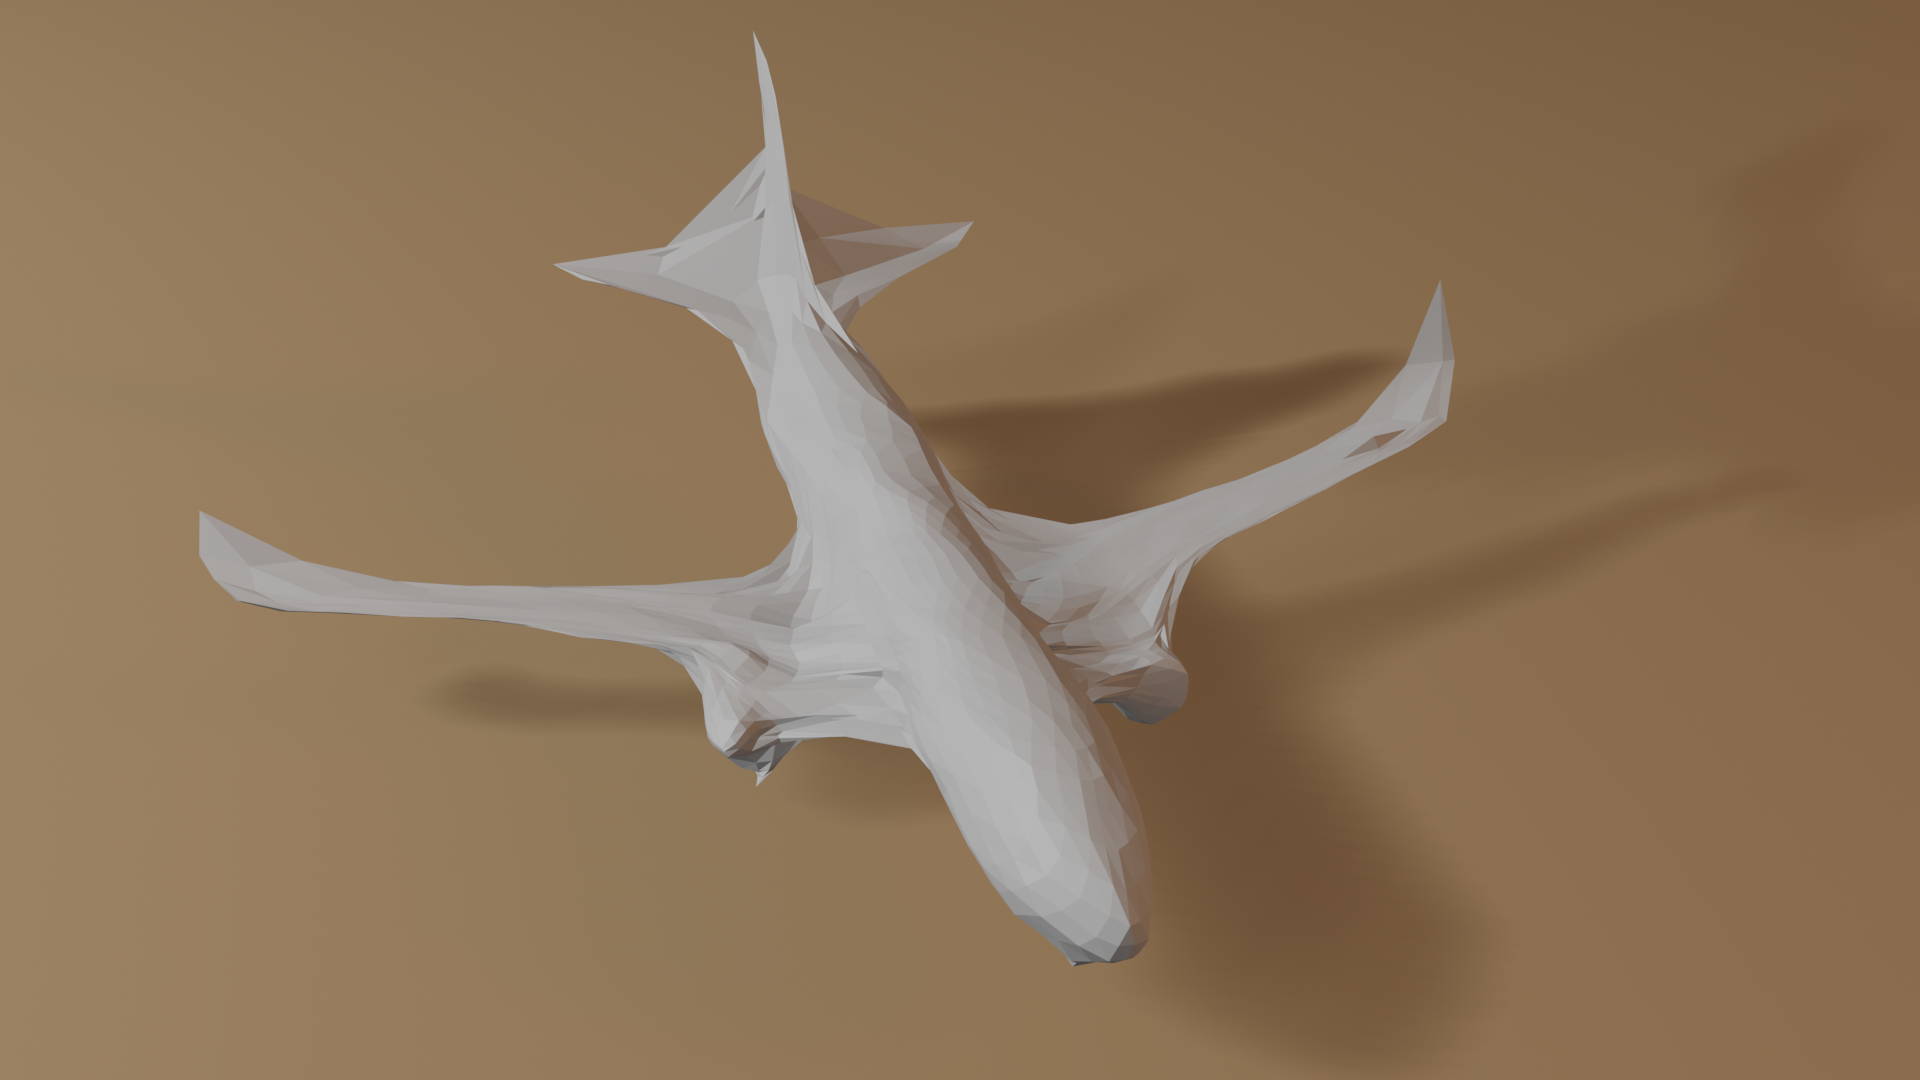
\includegraphics[width=0.32\textwidth]{c1_1024_airplane_1.png}}
  \subfloat[Configuration $\mathcal{C}_2$.\label{fig:1c}]{\includegraphics[width=0.32\textwidth]{c2_1024_airplane_1.png}}\\
  \subfloat[Sampled point cloud from ground truth mesh.\label{fig:1d}]{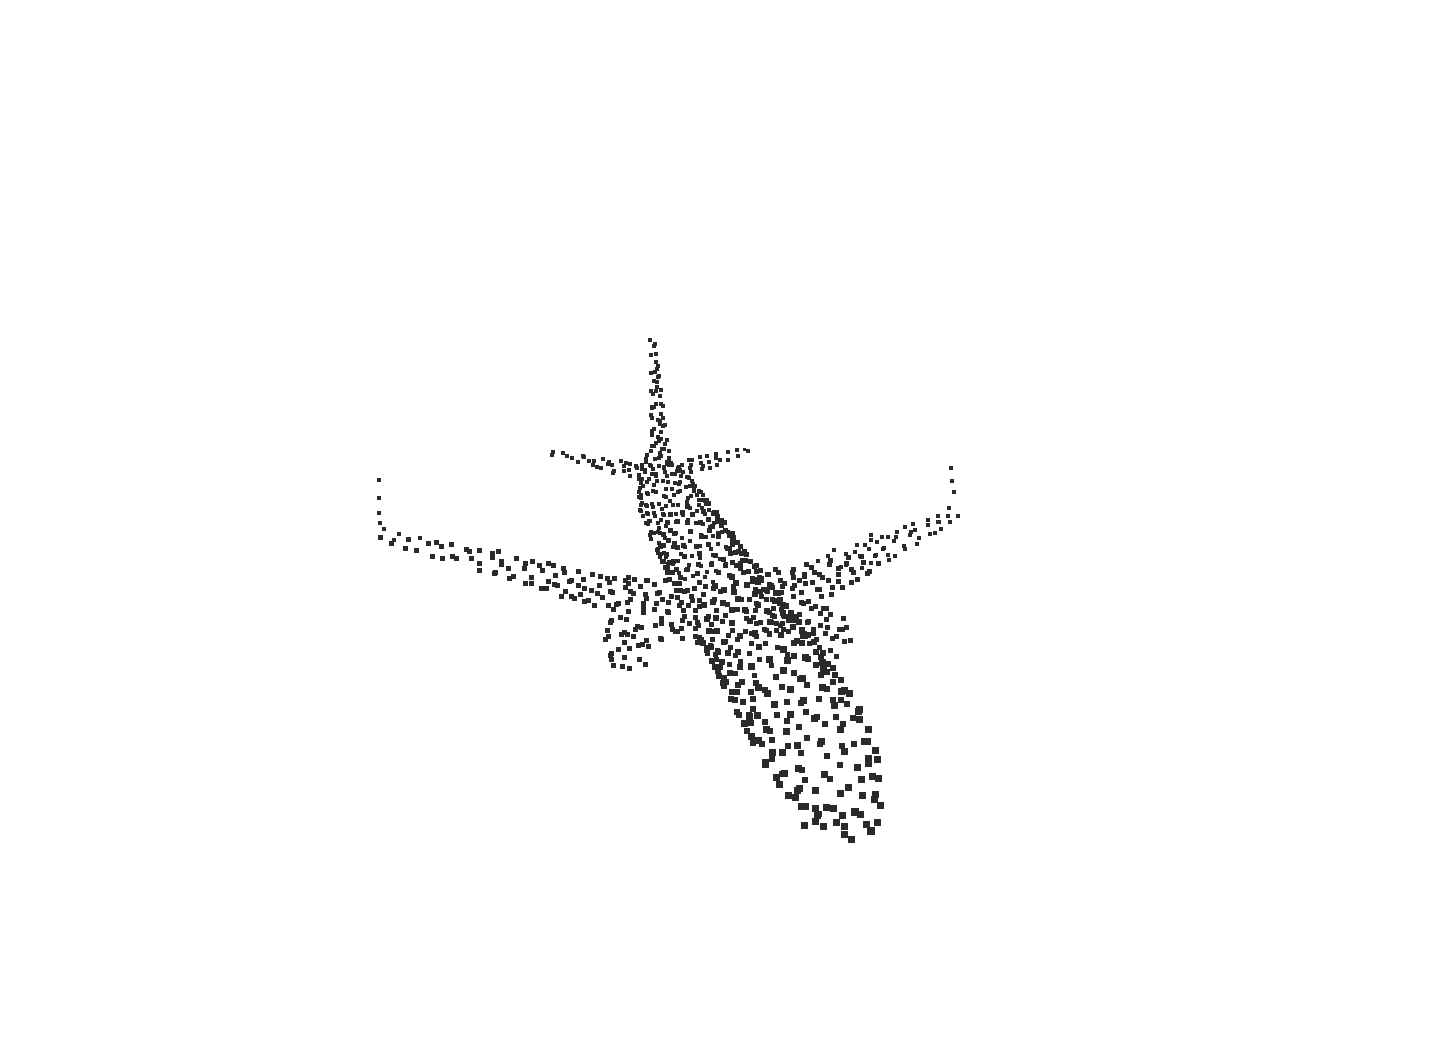
\includegraphics[width=0.32\textwidth]{airplane_1_pc.png}}
  \subfloat[Configuration $\mathcal{C}_3$.\label{fig:1e}]{\includegraphics[width=0.32\textwidth]{c3_1024_airplane_1.png}}
  \subfloat[Configuration $\mathcal{C}_4$.\label{fig:1f}]{\includegraphics[width=0.32\textwidth]{c4_1024_airplane_1.png}}\\
  \subfloat[Reconstrucion with \emph{BPA}.\label{fig:1g}]{\includegraphics[width=0.32\textwidth]{airplane_bpa_1024.png}}
  \subfloat[Reconstruction with \emph{IFM}.\label{fig:1h}]{\includegraphics[width=0.32\textwidth]{ifm_1024_airplane_1.png}}
  \subfloat[Reconstruction with \emph{DMC}.\label{fig:1i}]{\includegraphics[width=0.32\textwidth]{dmc_airplane.png}}
  \caption{Reconstruction of an airplane from point cloud with 1024 samples.} \label{fig:1}
\end{figure}

\begin{figure}[htbp]
  \centering
  \subfloat[Ground truth mesh.\label{fig:2a}]{\includegraphics[width=0.32\textwidth]{gt_chair_1.png}}
  \subfloat[Configuration $\mathcal{C}_1$.\label{fig:2b}]{\includegraphics[width=0.32\textwidth]{c1_1024_chair_1.png}}
  \subfloat[Configuration $\mathcal{C}_2$.\label{fig:2c}]{\includegraphics[width=0.32\textwidth]{c2_1024_chair_1.png}}\\
  \subfloat[Configuration $\mathcal{C}_3$.\label{fig:2d}]{\includegraphics[width=0.32\textwidth]{c3_1024_chair_1.png}}
  \subfloat[Configuration $\mathcal{C}_4$.\label{fig:2epro}]{\includegraphics[width=0.32\textwidth]{c4_1024_chair_1.png}}
  \caption{Reconstruction of a chair from point cloud with 1024 samples.} \label{fig:2}
\end{figure}

\begin{figure}[htbp]
  \centering
  \subfloat[Ground truth mesh.\label{fig:3a}]{\includegraphics[width=0.32\textwidth]{gt_guitar_1.png}}
  \subfloat[Configuration $\mathcal{C}_1$.\label{fig:3b}]{\includegraphics[width=0.32\textwidth]{c1_1024_guitar_1.png}}
  \subfloat[Configuration $\mathcal{C}_2$.\label{fig:3c}]{\includegraphics[width=0.32\textwidth]{c2_1024_guitar_1.png}}\\
  \subfloat[Sampled point cloud from ground truth mesh.\label{fig:3d}]{\includegraphics[width=0.32\textwidth]{guitar_pc00.png}}
  \subfloat[Configuration $\mathcal{C}_3$.\label{fig:3e}]{\includegraphics[width=0.32\textwidth]{c3_1024_guitar_1.png}}
  \subfloat[Configuration $\mathcal{C}_4$.\label{fig:3f}]{\includegraphics[width=0.32\textwidth]{c4_1024_guitar_1.png}}\\
  \subfloat[\emph{IFM} guitar reconstruction.\label{fig:3g}]{\includegraphics[width=0.32\textwidth]{ifm_1024_guitar_1.png}}
  \subfloat[\emph{DMC} guitar reconstruction.\label{fig:3h}]{\includegraphics[width=0.32\textwidth]{dmc_guitar.png}}
  \caption{Reconstruction of a guitar from point cloud with 1024 samples.} \label{fig:3}
\end{figure}
\begin{figure}[htbp]
  \centering
  \subfloat[Ground truth mesh.\label{fig:4a}]{\includegraphics[width=0.32\textwidth]{gt_bowl_1.png}}
  \subfloat[Configuration $\mathcal{C}_1$.\label{fig:4b}]{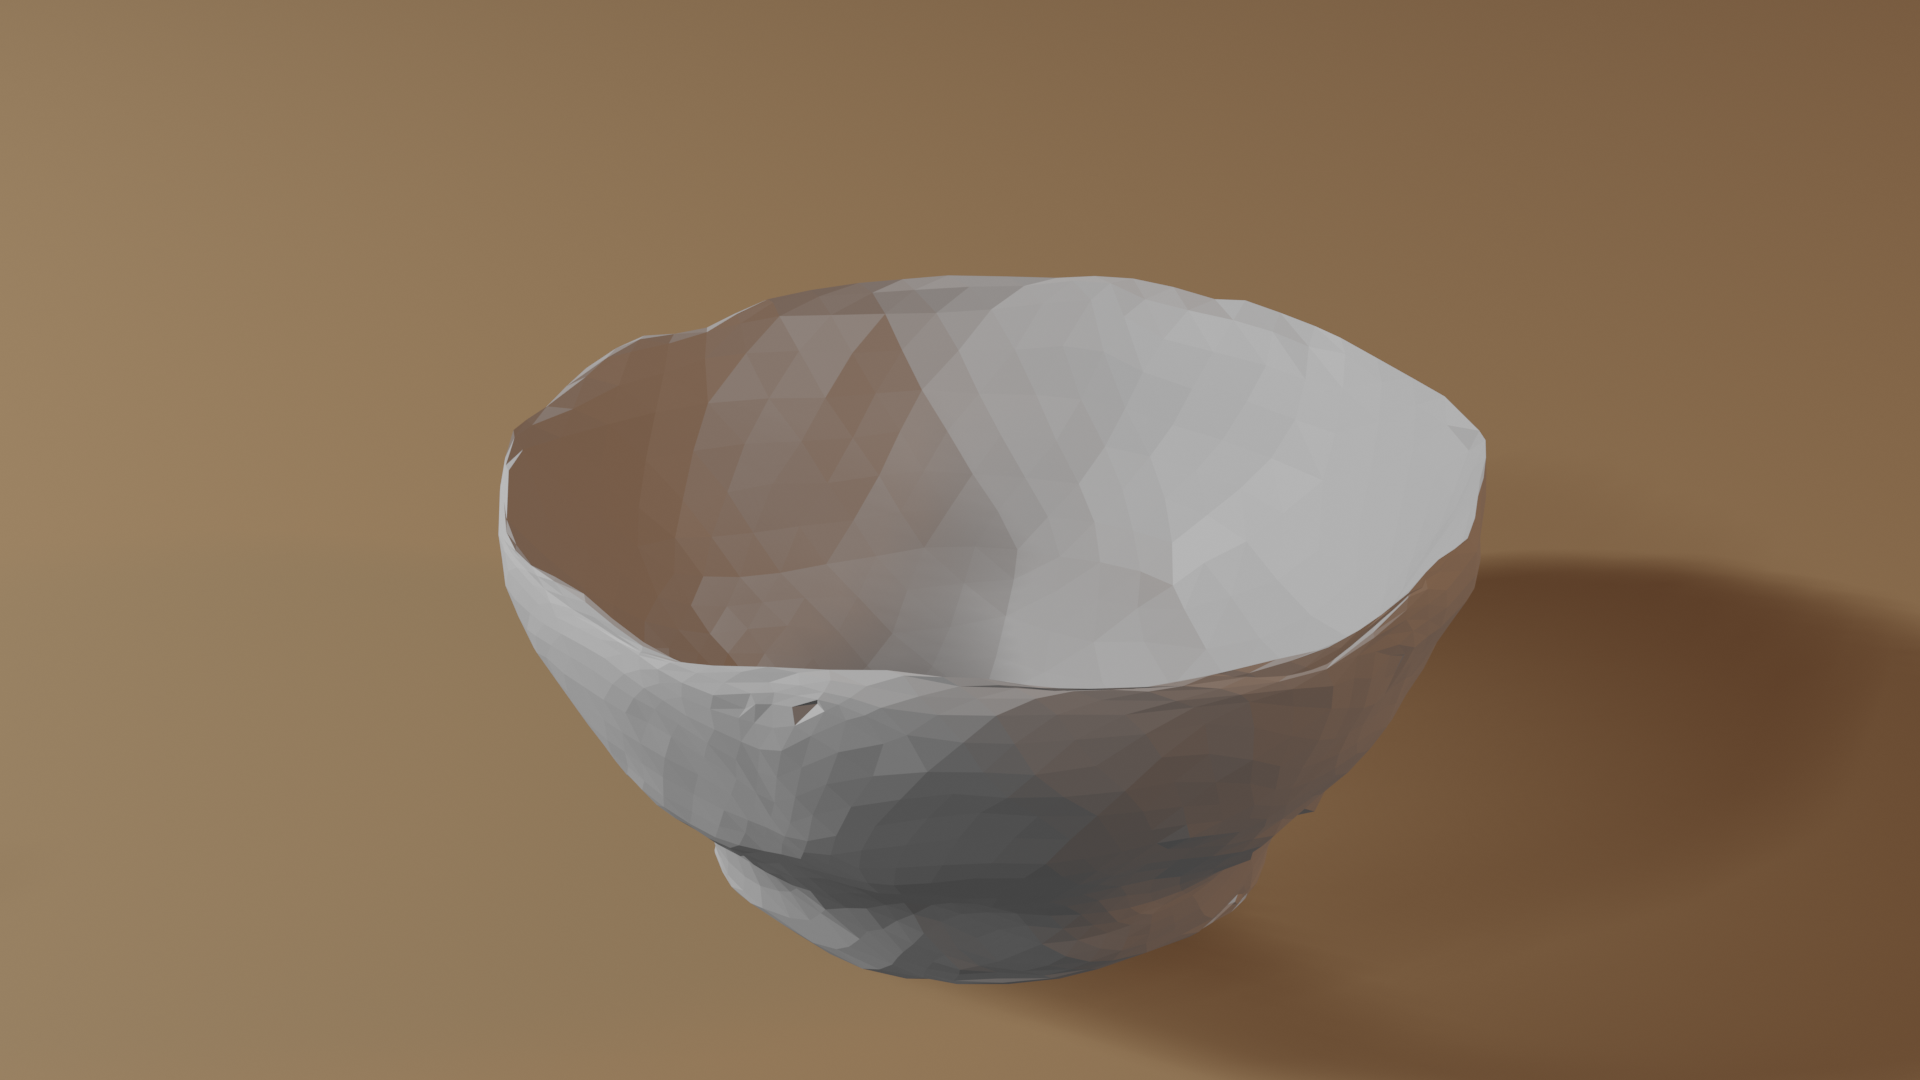
\includegraphics[width=0.32\textwidth]{c1_1024_bowl_1.png}}
  \subfloat[Configuration $\mathcal{C}_2$.\label{fig:4c}]{\includegraphics[width=0.32\textwidth]{c2_1024_bowl_1.png}}\\
  \subfloat[Reconstruction with \emph{DMC}\label{fig:4d}]{\includegraphics[width=0.32\textwidth]{dmc_bowl.png}}
  \subfloat[Configuration $\mathcal{C}_3$.\label{fig:4e}]{\includegraphics[width=0.32\textwidth]{c3_1024_bowl_1.png}}
  \subfloat[Configuration $\mathcal{C}_4$.\label{fig:4f}]{\includegraphics[width=0.32\textwidth]{c4_1024_bowl_1.png}}
  \caption{Reconstruction of a bowl from point cloud with 1024 samples.} \label{fig:4}
\end{figure}

  The last row depicts reconstructions with \emph{BPA}, \emph{IFM}, and \emph{DMC}. While the reconstruction with configuration 
  $\mathcal{C}_1$ represents the most interesting features of the airplane, especially the small winglets, it still has some errors. 
  One of the errors is at the rear of the plane with an edge dangling in the air, spanning over it. The same error happens with configuration
  $\mathcal{C}_3$ and $\mathcal{C}_4$ too. Configuration $\mathcal{C}_2$ seems to represent the airplane's features the best, though the least
  smooth of all reconstructions. As seen in figures \ref{fig:1f} and \ref{fig:2c}, configuration $\mathcal{C}_2$ is generally depicting the ground
    truth mesh in a good way, though not smooth.
  Considering other reconstruction methods, different problems, but also positives can be seen. \emph{BPA} reproduces smooth results as seen 
  in figure \ref{fig:1g}, while \emph{IFM} does not perform as well on low samples (~256 and 1024~) as seen in figure \ref{fig:1h}. Generally 
  \emph{DMC} does not perform good either as seen in figures \ref{fig:1i} and \ref{fig:3h}.

  Similarly, figure \ref{fig:2} through \ref{fig:5} show reconstructions with the same configurations $\mathcal{C}_i$ from $\mathcal{N}_{recon}$,
  but with an object from the \emph{categories} \emph{chair}, \emph{guitar}, \emph{bowl}. These \emph{categories} were included
  in the training set of $\mathcal{N}_{recon}$, though every reconstructed object sample originate from a test set, and thus have not be seen
  during the training stage.
  Similar behavior of the four network configurations, as described above, can be seen again, including the spanning of edges over empty space,
  like in figure \ref{fig:2d}, between the legs of the chair.


% 256
\begin{figure}[htbp]
  \centering
  \centering
  \subfloat[Ground truth mesh.\label{fig:5a}]{\includegraphics[width=0.5\textwidth]{gt_chair_256_1.png}}
  \subfloat[Ground truth mesh.\label{fig:5b}]{\includegraphics[width=0.5\textwidth]{gt_chair_7500.png}}\\
  \subfloat[Sampled point cloud from ground truth mesh.\label{fig:5b}]{\includegraphics[width=0.5\textwidth]{chair_256_pc06.png}}
  \subfloat[Sampled point cloud from ground truth mesh.\label{fig:5c}]{\includegraphics[width=0.5\textwidth]{chair_256_pc00.png}}\\
  \subfloat[Configuration $\mathcal{C}_1$.\label{fig:5d}]{\includegraphics[width=0.5\textwidth]{c1_256_chair_1.png}}
  \subfloat[Configuration $\mathcal{C}_2$.\label{fig:5e}]{\includegraphics[width=0.5\textwidth]{c1_256_chair_2.png}}\\
  \caption{Reconstruction of chairs from point cloud with 256 samples.} \label{fig:5}
\end{figure}
\begin{figure}[htbp]
  \centering
  \subfloat[Ground truth mesh.\label{fig:51a}]{\includegraphics[width=0.5\textwidth]{gt_car_1.png}}
  \subfloat[Sampled point cloud from ground truth mesh.\label{fig:51b}]{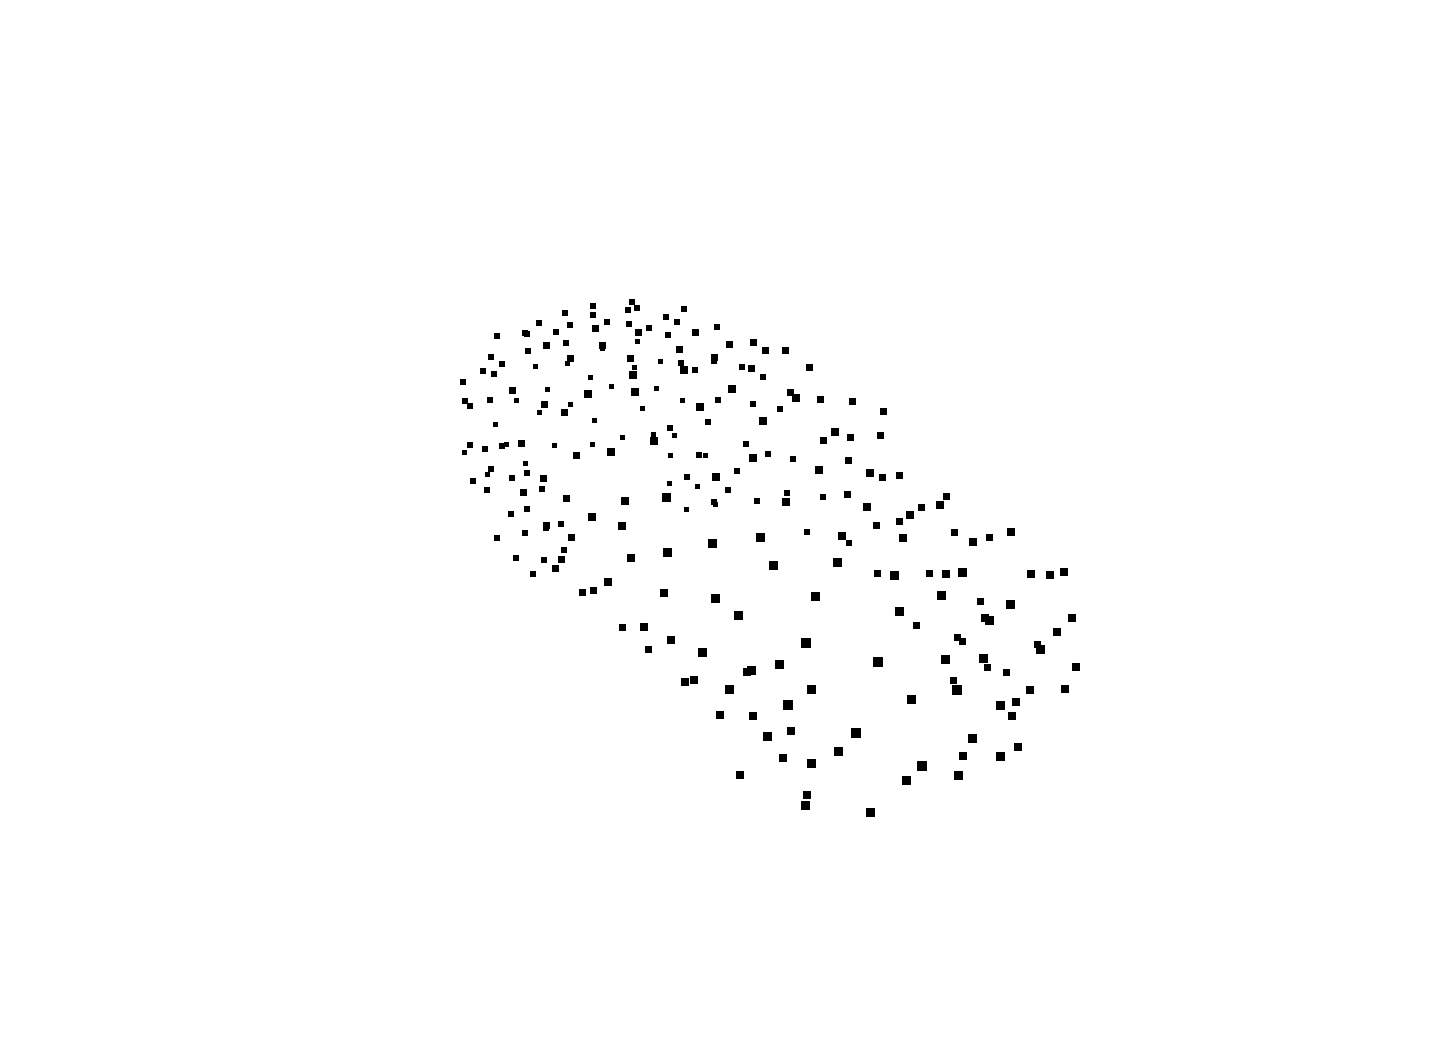
\includegraphics[width=0.5\textwidth]{car_pc05.png}}\\
  \subfloat[Configuration $\mathcal{C}_1$.\label{fig:51c}]{\includegraphics[width=0.5\textwidth]{c1_256_car_1.png}}
  \subfloat[Reconstruction of car with \emph{DMC},.\label{fig:51d}]{\includegraphics[width=0.5\textwidth]{dmc_car.png}}
  \caption{Reconstruction of a car from point cloud with 256 samples.} \label{fig:51}
\end{figure}
\begin{figure}[htbp]
  \centering
  \subfloat[Ground truth mesh.\label{fig:52a}]{\includegraphics[width=0.33\textwidth]{gt_256_toilet.png}}
  \subfloat[Configuration $\mathcal{C}_1$.\label{fig:52b}]{\includegraphics[width=0.33\textwidth]{c1_256_toilet.png}}
  \subfloat[Reconstruction with \emph{BPA}\label{fig:52c}]{\includegraphics[width=0.33\textwidth]{bpa_256_toilet.png}}
  \caption{Reconstruction of a toilet from point cloud with 256 samples.} \label{fig:52}
\end{figure}
  Figures \ref{fig:5} and \ref{fig:51} show reconstruction with a sample size of 256. Depicted are reconstructions with configurations
  $\mathcal{C}_1$ and $\mathcal{C}_2$ 
  and their corresponding ground truth mesh and sampled point cloud.
  While still able to reconstruct the general shape of the object, the spanning problem is still visible.
  Additionally, \emph{DMC} is not able to handle bigger empty spaces in the sparse cloud well enough to create a proper reconstruction,
  as seen in figure \ref{fig:51d}.


  \begin{figure}[htbp]
    \centering
    \subfloat[Ground truth mesh.\label{fig:6a}]{\includegraphics[width=0.4\textwidth]{gt_chair_7500.png}}
    \subfloat[Sampled point cloud from ground truth mesh.\label{fig:6b}]{\includegraphics[width=0.4\textwidth]{chair_pc00.png}}\\
    \subfloat[Configuration $\mathcal{C}_1$.\label{fig:6c}]{\includegraphics[width=0.4\textwidth]{c1_7500_chair_2.png}}
    \subfloat[Configuration $\mathcal{C}_4$.\label{fig:6d}]{\includegraphics[width=0.4\textwidth]{c4_7500_chair_2.png}}
    \caption{Reconstruction of a chair from point cloud with 7500 samples.} \label{fig:6}
  \end{figure}
  \begin{figure}[htbp]
    \centering
    \subfloat[Ground truth mesh.\label{fig:61a}]{\includegraphics[width=0.4\textwidth]{gt_airplane_7500.png}}
    \subfloat[Samples pointc loud from ground truth mesh.\label{fig:6d}]{\includegraphics[width=0.4\textwidth]{plane2_pc04.png}}\\
    \subfloat[Configuration $\mathcal{C}_1$.\label{fig:6e}]{\includegraphics[width=0.4\textwidth]{c4_7500_airplane_2.png}}
    \subfloat[Configuration $\mathcal{C}_4$.\label{fig:6f}]{\includegraphics[width=0.4\textwidth]{c1_7500_airplane_2.png}}
    \caption{Reconstruction of an airplane from point cloud with 7500 samples.} \label{fig:61}
  \end{figure}
  
  Figures \ref{fig:6} and \ref{fig:61} show reconstruction of a chair and an airplane from 7500 samples. Depicted are configurations 
  $\mathcal{C}_1$ and $\mathcal{C}_4$.


% 7500

%256-1024-7500
\begin{figure}[htbp]
  \centering
  \subfloat[Ground truth mesh.\label{fig:7a}]{\includegraphics[width=0.5\textwidth]{gt_airplane_7500.png}}
  \subfloat[$\mathcal{C}_1$ with sample size 256.\label{fig:7b}]{\includegraphics[width=0.5\textwidth]{c1_256_airplane_2.png}}\\
  \subfloat[$\mathcal{C}_1$ with sample size 1024.\label{fig:7c}]{\includegraphics[width=0.5\textwidth]{c1_1024_airplane_2.png}}
  \subfloat[$\mathcal{C}_1$ with sample size 7500.\label{fig:7d}]{\includegraphics[width=0.5\textwidth]{c4_7500_airplane_2.png}}\\
  \subfloat[\emph{BPA} with sample size 7500.\label{fig:7e}]{\includegraphics[width=0.5\textwidth]{airplane2_ifm_7500.png}}
  \subfloat[\emph{IFM} with sample size 7500.\label{fig:7f}]{\includegraphics[width=0.5\textwidth]{airplane2_bpa_7500.png}}
  \caption{Reconstruction of an airplane with different sample sizes, but the same configuration $\mathcal{C}_1$.} \label{fig:7}
\end{figure}

  For easier comparisons, figure \ref{fig:7} shows the reconstruction of the same airplane with configuration $\mathcal{C}_1$ but with
  different sample sizes, as well as reconstructions from \emph{BPA} and \emph{IFM} with the same sample size, showing their ostensible
  superiority with more samples.


  \begin{figure}[htbp]
    \centering
    \subfloat[Noisy airplane 1.\label{fig:81a}]{\includegraphics[width=0.5\textwidth]{c1_1024_noise_airplane_1.png}}
    \subfloat[Noisy airplane 2.\label{fig:81b}]{\includegraphics[width=0.5\textwidth]{c1_1024_noise_airplane_2.png}}\\
    \subfloat[Noisy airplane 3.\label{fig:81c}]{\includegraphics[width=0.5\textwidth]{c1_1024_noise_airplane_3.png}}
    \subfloat[Noisy airplane 4.\label{fig:81d}]{\includegraphics[width=0.5\textwidth]{c1_1024_noise_airplane_4.png}}
    \caption{Reconstruction of airplanes with $\mathcal{C}_1$ from noisy point cloud with noise factor of $0.01$. } \label{fig:81}
  \end{figure}
  Next, in figure \ref{fig:81}, reconstruction of airplanes and with configuration $\mathcal{C}_1$ can be seen. Each point in the point 
  cloud has random
  jitter noise between $-0.01$ and $0.01$ added on top of it.


% generalization
\begin{figure}[htbp]
  \centering
  \subfloat[Ground truth mesh.\label{fig:8a}]{\includegraphics[width=0.32\textwidth]{gt_person_1.png}}
  \subfloat[$\mathcal{C}_1$.\label{fig:8b}]{\includegraphics[width=0.32\textwidth]{c1_1024_person_1.png}}
  \subfloat[$\mathcal{C}_2$.\label{fig:8c}]{\includegraphics[width=0.32\textwidth]{c2_1024_person_1.png}}\\
  \subfloat[Sampled point cloud from ground truth mesh.\label{fig:8d}]{\includegraphics[width=0.32\textwidth]{person_pc00.png}}
  \subfloat[$\mathcal{C}_3$.\label{fig:8e}]{\includegraphics[width=0.32\textwidth]{c3_1024_person_1.png}}
  \subfloat[$\mathcal{C}_4$.\label{fig:8f}]{\includegraphics[width=0.32\textwidth]{c4_1024_person_1.png}}
  \caption{Reconstruction from point clouds of untrained category \emph{person}.} \label{fig:8}
\end{figure}
\begin{figure}[htbp]
  \centering
  \subfloat[$\mathcal{C}_1$.\label{fig:9a}]{\includegraphics[width=0.5\textwidth]{c1_1024_bathtub_1.png}}
  \subfloat[$\mathcal{C}_2$.\label{fig:9b}]{\includegraphics[width=0.5\textwidth]{c2_1024_bathtub_1.png}}\\
  \subfloat[$\mathcal{C}_3$.\label{fig:9c}]{\includegraphics[width=0.5\textwidth]{c3_1024_bathtub_1.png}}
  \subfloat[$\mathcal{C}_4$.\label{fig:9d}]{\includegraphics[width=0.5\textwidth]{c4_1024_bathtub_1.png}}
  \caption{Reconstruction from point clouds of untrained category \emph{bathutb}.} \label{fig:9}
\end{figure}
  Finally, figures \ref{fig:8} and figure \ref{fig:9} show the reconstruction of a person and a bathtub, based on point cloud samples 
  which $\mathcal{N}_{recon}$ has not been trained with.

